\section{Архитектура базы данных Dictorpus} \label{sect_arch_db}

\begin{landscape}

\begin{figure}
    \centering
    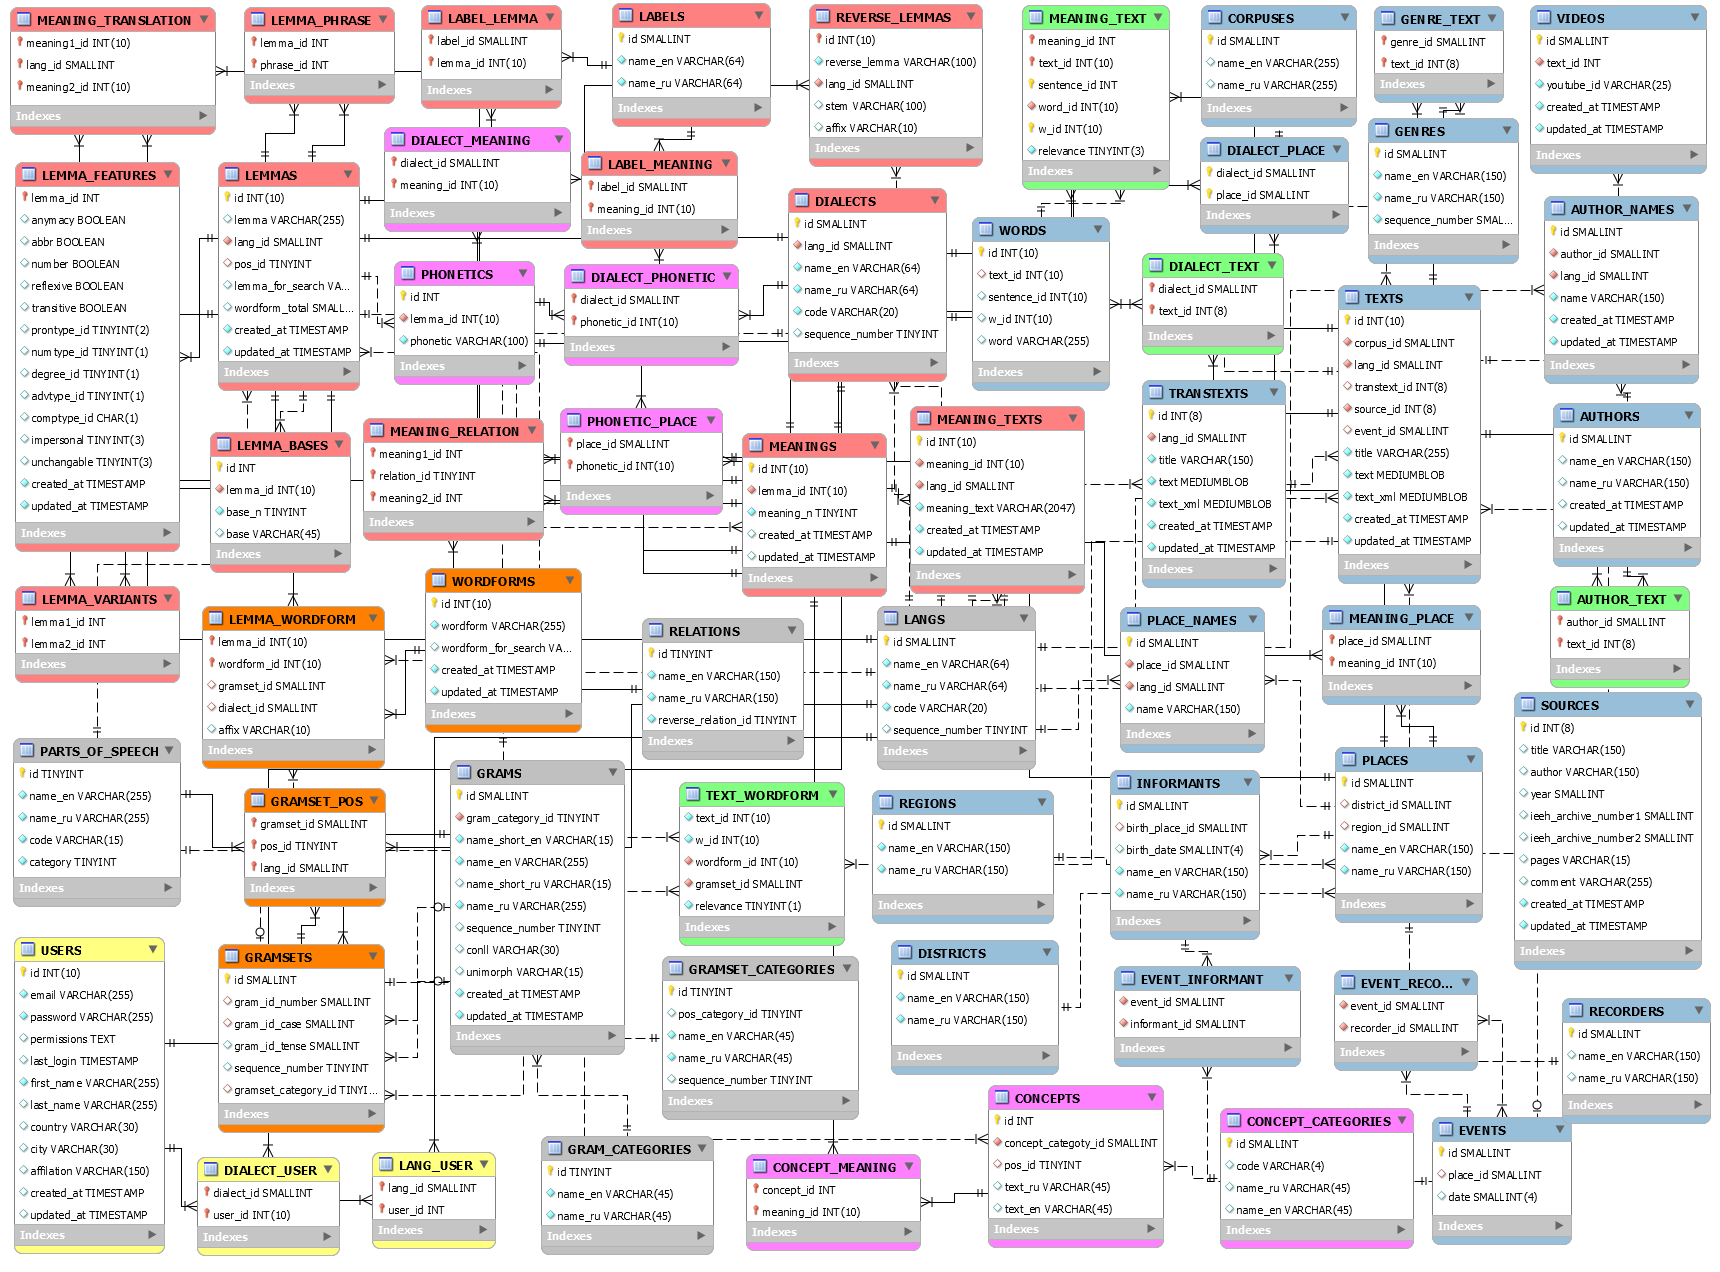
\includegraphics[width=1.1\textwidth,keepaspectratio=true]{db/vepkar_db_scheme.png}
   \caption{Структура БД Dictorpus. Данные на 13 февраля 2021 г.  См. схему: \url{https://bit.ly/3aftLIl}.} 
   \label{fig:vepkar_db_scheme}
\end{figure}

\colorindicator{tab:pink}{розовые}~--- со словарными статьями;
\colorindicator{tab:magenta}{пурпурные}~--- с фонетикой и понятиями;
\colorindicator{tab:orange}{оранжевые}~--- со словоформами;
\colorindicator{tab:yellow}{жёлтые}~--- с пользователями;
\colorindicator{tab:cyan}{голубые}~--- с текстами;
\colorindicator{tab:grey}{серые}~--- общие справочники.
\end{landscape}